\documentclass{beamer}
\usetheme[style=plain]{uu}

\usepackage{graphicx}
\usepackage{mathtools}
\usepackage{amssymb}
\usepackage{hyperref}
\usepackage{color}
\usepackage{float}

%% unicode support, for text and code :)
\usepackage[utf8x]{inputenc}
\usepackage{ucs}
\usepackage{autofe}


%% Haskell syntax highlighting and code font
\usepackage{minted}
\usepackage{fancyvrb}
\usepackage{inconsolata}
\usemintedstyle{default}

\newmint{haskell}{mathescape,fontfamily=tt}
\newmintedfile{haskell}{xleftmargin=20pt,mathescape,fontfamily=tt}

\newminted{haskell}{xleftmargin=20pt,gobble=8,mathescape,fontfamily=tt}
\newmint{coq}{mathescape,fontfamily=tt}

\newmintedfile{coq}{xleftmargin=20pt,mathescape,fontfamily=tt}
\newminted{coq}{gxleftmargin=20pt,obble=8,mathescape,fontfamily=tt}



%% Metainformation
%% PDF stuff
\usepackage{datetime}
\usepackage{ifpdf}
\ifpdf
\pdfinfo{
    /Author (Joao Paulo Pizani Flor)
    /Title (Comparing functional EDSLs for hardware description)
    /Keywords (Hardware verification, Functional Programming, Hardware design, Dependently-typed programming, Coq, Lava, ForSyDe, Haskell, Coquet)
    /CreationDate (D:\pdfdate)
}
\fi

\title[Comparing functional EDSLs for hardware description]{Comparing functional Embedded Domain-Specific Languages for hardware description}

\date{February 13th, 2014}

\author[Pizani Flor]
{
    João Paulo Pizani Flor
}

\institute[Utrecht University]
{
    Department of Information and Computing Sciences,
    Utrecht University
}

\subject{Function Programming, Hardware verification, Haskell, Coq, Lava, Coquet, ForSyDe}




\begin{document}

%% The document itself
    \begin{frame}
        \titlepage
    \end{frame}

    \begin{frame}
        \frametitle{Table of Contents}
        \tableofcontents
    \end{frame}



    \section{Introduction}
    \label{sec:introduction}
        \frame{\sectionpage}

        \subsection{Hardware design}
        \label{subsec:hardware-design}
            \begin{frame}
                \frametitle{Hardware design}
            \end{frame}


        \subsection{Domain-Specific Languages}
        \label{subsec:domain-specific-languages}
            % deep-embedded / shallow embedded
            \begin{frame}
                \frametitle{Domain-Specific Languages}

                \par{A computer language (turing-complete or \emph{not}) targeting a \emph{specific application domain.}}
                \par{\textbf{Example DSLs:}}
                \begin{itemize}
                    \item SQL (database queries)
                    \item CSS (document formatting)
                    \item MATLAB (Matrix programming)
                    \item VHDL (Hardware description)
                \end{itemize}

                \pause

                \par{A DSL can also be \emph{embedded} in a general-purpose language.}
                \par{\textbf{Example EDSLs:}}
                \begin{itemize}
                    \item Boost.Proto (C++ / parser combinators)
                    \item Diagrams (Haskell / programmatic drawing)
                    \item Parsec (Haskell / parser combinators)
                \end{itemize}
            \end{frame}

            \begin{frame}[fragile]
                \frametitle{Example of an EDSL: \texttt{Parsec}}

                A simple parser for a "Game of Life"-like input format:
                \haskellfile{code/parsec-example.hs}
\end{frame}


        \subsection{Hardware EDSLs}
        \label{subsec:hardware-edsls}
            \begin{frame}
                \frametitle{Hardware EDSLs}
                An EDSL used for hardware design-related tasks. Can encompass:

                \begin{itemize}
                    \item Modelling / description
                    \item Simulation (validation)
                    \item Formal verification
                    \item Synthesis to other (lower-level) languages
                \end{itemize}
            \end{frame}

            \begin{frame}
                \frametitle{Example of a hardware EDSL}

                Some Lava code\ldots
            \end{frame}



    \section{Analyzed EDSLs}
    \label{sec:analyzed-edsls}
        \frame{\sectionpage}

        \subsection{Choice criteria}
        \label{subsec:edsls-choice-criteria}
            \begin{frame}
                \frametitle{Choice criteria}
            \end{frame}


        \subsection{Chosen EDSLs}
        \label{subsec:chosen-edsls}
            \begin{frame}
                \frametitle{Chosen EDSLs}
                The language we chose to evaluate, with the respective host language, were:

                \begin{itemize}
                    \item Lava (Haskell - \texttt{chalmers-lava} \emph{dialect})
                    \item ForSyDe (Haskell)
                    \item Coquet (Coq)
                \end{itemize}
            \end{frame}

        \subsection{Evaluation criteria}
        \label{subsec:evaluation-criteria}
            \begin{frame}
                \frametitle{Evaluation criteria}

                \begin{itemize}
                    \item Simulation
                    \item Verification
                    \item Genericity
                    \item Depth of embedding
                    \item Tool integration
                    \item Extensibility
                \end{itemize}
            \end{frame}



    \section{Modeled Circuits}
    \label{sec:modeled-circuits}
        \frame{\sectionpage}

        \subsection{Choice}
        \label{subsec:circuit-choice-criteria}
            \begin{frame}
                \frametitle{Choice criteria}

                \begin{itemize}
                    \item Not too simple, not too complex
                    \item Familiar to any hardware designer
                        \begin{itemize}
                            \item No signal processing, etc.
                        \end{itemize}
                    \item Well-defined, pre-specification
                        \begin{itemize}
                            \item Results to verify the models against
                        \end{itemize}
                \end{itemize}
            \end{frame}

            \begin{frame}
                \frametitle{Chosen circuits}

                \par{We cherry-picked circuits from the book ``Elements of Computing Systems'',
                    as they satisfied all of our demands.}

                \begin{figure}[h!]
                    \includegraphics[width=0.5\textwidth]{imgs/book-cover-elements.jpg}
                    \caption{``Elements of Computing Systems'' - Nisan, Schocken, \newline
                        available at \url{http://www.nand2tetris.org}.
                        \label{fig:book-cover-elements}
                    }
                \end{figure}
            \end{frame}

            \begin{frame}
                \frametitle{Chosen circuits}

                \begin{description}
                    \item[Circuit 1] A 2-input, 16-bit-wide, simple ALU
                    \item[Circuit 2] A 64-word long, 16-bit wide memory block
                    \item[Circuit 3] An \emph{extremely} reduced instruction set CPU,
                        the \emph{Hack} CPU.
                \end{description}
                \vspace{0.05\textwidth}

                \par{Let's take a quick look at each of these circuit's specification\ldots}
            \end{frame}


        \subsection{ALU}
        \label{subsec:alu}
            \begin{frame}
                \frametitle{Circuit 1: ALU}

                \par{Some of the circuit's key characteristics:}

                \begin{itemize}
                    \item 2 \emph{operand inputs} and 1 \emph{operand output}, each 16-bit wide
                    \item 1 \emph{output flag}
                    \item Can execute 18 different \emph{functions}, among which:
                        \begin{itemize}
                            \item Addition, subtraction
                            \item Bitwise AND / OR
                            \item Constant outputs
                            \item Addition of constants to an operand
                            \item Sign inversion
                        \end{itemize}
                \end{itemize}
            \end{frame}

            \begin{frame}
                \frametitle{Circuit 1: block diagram}

                \begin{figure}[h!]
                    \centerline{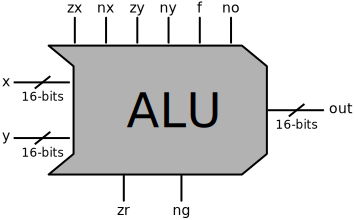
\includegraphics[width=0.6\textwidth]{imgs/alu-block.pdf}}
                    \caption{Input/Output ports of \emph{circuit 1}, the ALU.
                        \label{fig:alu-block}}
                \end{figure}
            \end{frame}

            \begin{frame}
                \frametitle{Circuit 1: Specification}

                \par{The behaviour of the ALU is specified by the values of the \emph{control bits} and flags:}

                \begin{description}
                    \item[\texttt{zx} and \texttt{zy}]
                        \emph{Zeroes} the \texttt{x} and \texttt{y} inputs, respectively
                    \item[\texttt{nx} and \texttt{ny}]
                        \emph{bitwise negation} in the \texttt{x} and \texttt{y} inputs
                    \item[\texttt{f}]
                        Selects the function to be applied: \newline
                        $f = 1$ for addition, $f = 0$ for bitwise AND
                    \item[\texttt{no}]
                        \emph{bitwise negation} on the output ALU output
                    \item[\texttt{zr} and \texttt{ng}]
                        The output \emph{flag} $\text{zr} = 1$ \emph{iff} the ALU output is zero.
                        $\text{ng} = 1$ \emph{iff} the output is negative.
                \end{description}

                \par{Operations such as bitwise OR, subtraction, etc. can be done by setting the control bits appropriately.}
            \end{frame}


        \subsection{Memory bank}
        \label{subsec:memory-bank}
            \begin{frame}
                \frametitle{Circuit 2: RAM64}

                \par{Some of the circuit's key characteristics:}

                \begin{itemize}
                    \item \emph{Sequential} circuit, with clock input
                    \item 64 memory words stored, each 16-bit wide
                    \item Address port has width $\log_{2} 64 = 16$ bit
                \end{itemize}
            \end{frame}

            \begin{frame}
                \frametitle{Circuit 2: block diagram}

                \begin{figure}[h!]
                    \centerline{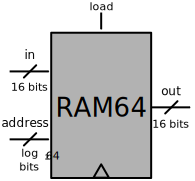
\includegraphics[width=0.45\textwidth]{imgs/ram-block.pdf}}
                    \caption{Input/Output ports of \emph{circuit 2}, the RAM64 block.
                        \label{fig:ram-block}}
                \end{figure}
            \end{frame}


        \subsection{CPU}
        \label{subsec:cpu}
            \begin{frame}
                \frametitle{CPU block diagram}

                \begin{figure}[h!]
                    \centerline{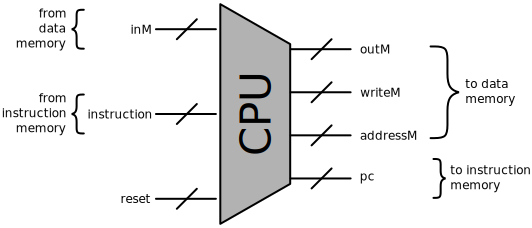
\includegraphics[width=1.0\textwidth]{imgs/cpu-block.pdf}}
                    \caption{Input/Output ports of \emph{circuit 3}, the \emph{Hack} CPU.
                        \label{fig:cpu-block}}
                \end{figure}
            \end{frame}



    \section{Analysis of the EDSLs}
    \label{sec:analysis-of-the-edsls}
        \frame{\sectionpage}

        \subsection{Lava}
        \label{subsec:lava}
            \begin{frame}
                \frametitle{Lava}
            \end{frame}

        \subsection{ForSyDe}
        \label{subsec:forsyde}
            \begin{frame}
                \frametitle{ForSyDe}
            \end{frame}

        \subsection{Coquet}
        \label{subsec:coquet}
            \begin{frame}
                \frametitle{Coquet}
            \end{frame}


    \section{Conclusions}
    \label{sec:conclusions}
        \frame{\sectionpage}

        \begin{frame}[plain]
            \begin{center}
                \par{\Huge{Thank you!}}
                \vspace{2.0cm}
                \par{\Huge{Questions?}}
            \end{center}
        \end{frame}


\end{document}
